\documentclass{article}
\usepackage{fullpage}
\usepackage{amsmath,amssymb}
\usepackage{cmll} %parr
\usepackage{tikz}
\usetikzlibrary{arrows,positioning,fit,petri,decorations.markings,shapes}

\newcommand{\meas}{\textrm{meas}}
\newcommand{\lolli}{\multimap}
\newcommand{\tensor}{\otimes} 
\newcommand{\proves}{\mathrel{\vdash}}
\newcommand{\qubit}[1]{\vert #1 \rangle}

\title{CIS 670, Spring 2014, Project Proposal}
\author{Jennifer Paykin and Antal Spector-Zabusky}

\begin{document}
\maketitle

This project aims to explore connections between the fields
of quantum computation and linear type systems. Much work has been
done exploring the connections between these two worlds. The connection
between quantum physics and category theory is addressed by 
Baez and Stay~\cite{baez2011physics}. On the other hand, 
Selinger and Valiron~\cite{selinger2009quantum} describe a lambda
calculus for quantum computation allowing them to write quantum
algorithms as terms in a higher-order term language. This project
will focus on two main areas: the idea of proof nets acting as circuit diagrams,
and the connection between classical linear logic (including the $\parr$ and $?$ operators)
and quantum computation.

\begin{figure}
\begin{center} 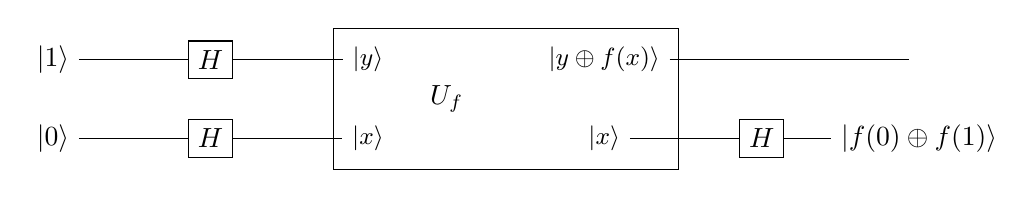
\begin{tikzpicture}
    \node (1) at (-3,1) {$\qubit{1}$} ;
    \node (0) at (-3,0) {$\qubit{0}$} ;
    \node[draw,rectangle] (H1) at (-1,1) {$H$} ;
    \node[draw,rectangle] (H2) at (-1,0) {$H$} ;
    \node[draw,rectangle] (H3) at ( 6,0) {$H$} ;
    \node (U) at (2,0.5) {$U_f$} ;
    \node (y1) at (1,1) {\small $\qubit{y}$} ;
    \node (x1) at (1,0) {\small $\qubit{x}$} ;
    \node (x2) at (4,0) {\small $\qubit{x}$} ;
    \node (y2) at (4,1) {\small $\qubit{y \oplus f(x)}$} ;
    \node (end) at (8,0) {$\qubit{f(0) \oplus f(1)}$} ;
    \node (empty) at (8,1) {} ;

    \node [draw, fit= (x1) (y1) (x2) (y2) (U)] {};

    \path[-] (1) edge node[align=center] {} (H1) ;
    \path[-] (0) edge node[align=center] {} (H2) ;
    \path[-] (H1) edge node[align=center] {} (y1) ;
    \path[-] (H2) edge node[align=center] {} (x1) ;
    \path[-] (x2) edge node[align=center] {} (H3) ;
    \path[-] (H3) edge node[align=center] {} (end) ;
    \path[-] (y2) edge node[align=center] {} (empty) ;
\end{tikzpicture} \end{center}
\caption{The Deutsch algorithm.
\label{fig:deutsch}}
\end{figure}

In quantum mechanics, circuit diagrams are one of the primary means
expressing computation. Without getting into specifics, 
Figure~\ref{fig:deutsch} is a circuit diagram describing the Deutsch algorithm.
The primitive Hadamard gate $H$ takes a qubit as input on the left
and outputs a qubit on the right. Furthermore, the diagram
$U_f$ shows how it is possible to compose circuits, which can be thought of as
black boxes; composition is done locally.

These same features can be seen in the theory of proof nets, in which composition
is a local operation interpreted by cut links. Proof nets in turn correspond
to typing derivations for the quantum lambda calculus. Blute and
Panangaden~\cite{blute2011proof} formalized the connection between
proof nets and Feynmann diagrams, which is a special case of circuit diagram.
We hope to make the connection intuitive without delving too far into the formal semantics
of these structures.

For linear logic, proof nets extend intuitively to cover the classical operator $\parr$.
We hope to explore this interpretation of $\parr$ as output-ports on the right-hand-side 
of circuit diagrams to find a natural interpretation of $\parr$ in quantum computation.
A similar question arises about the nature of the duality operation $(-)^\bot$,
which has a natural interpretation as a functor in quantum physics, but has not been
widely used in quantum lambda calculi.


\bibliographystyle{plain}
\bibliography{bibliography}

\end{document}


\begin{enumerate}
    \item Interpretation of $\parr$
    \item Circuit diagrams, proof nets, and lambda calculi
    \item Writing example programs
    \item quantum physics: compact symmetric monoidal category \cite{baez2011physics}
    \item qubit as $\bot \parr \bot$? bit as $1 \oplus 1$? Therefore
    $\meas : \bot \parr \bot \lolli (1 \oplus 1)$.
    \item If Hilbert spaces are compact, that means $\parr = \tensor$ 
    Perhaps we can write something that looks like a classical sequent
    calculus, but where the comma on right is $\tensor$? Or maybe just
    add a rule? ---OR, does compact not mean compact closed?
    \item Nope--compact just means every object has both a left and right dual
    \cite{baez2011physics}
    \item Does compact imply *-autonomous? ie are hilbert spaces *-autonomous?
    \item $1 \oplus 1 \proves !(1 \oplus 1)$ but 
    $\bot \parr \bot \not\proves !(bot \parr \bot)$
\end{enumerate}
